\section{Introduction}
\label{sec:introduction}

<<<<<<< HEAD
\par The goal of this laboratory assignment was to optimize a given audio amplifier, and doing both the theoretical and simulation analysis. The architecture of the given circuit can be seen in the following picture.
=======
\par The goal of this laboratory assignment was to build a BandPass Filter (BPF) with the following specifications: central frequency at 1MHz and gain at central frequency at 40dB, using an Operational Amplifier. In our case, we chose to use the non-inverting amplifier, as the objetive was only to amplify the sginal without inverting it. In order to optimize the amplifier, both the theoretical and simulation analysis were done. The architecture of the given circuit can be seen in the following picture.
>>>>>>> d0b080297fc0b7e965087175cb535c02ef7a19c1

\begin{figure}[H] \centering
	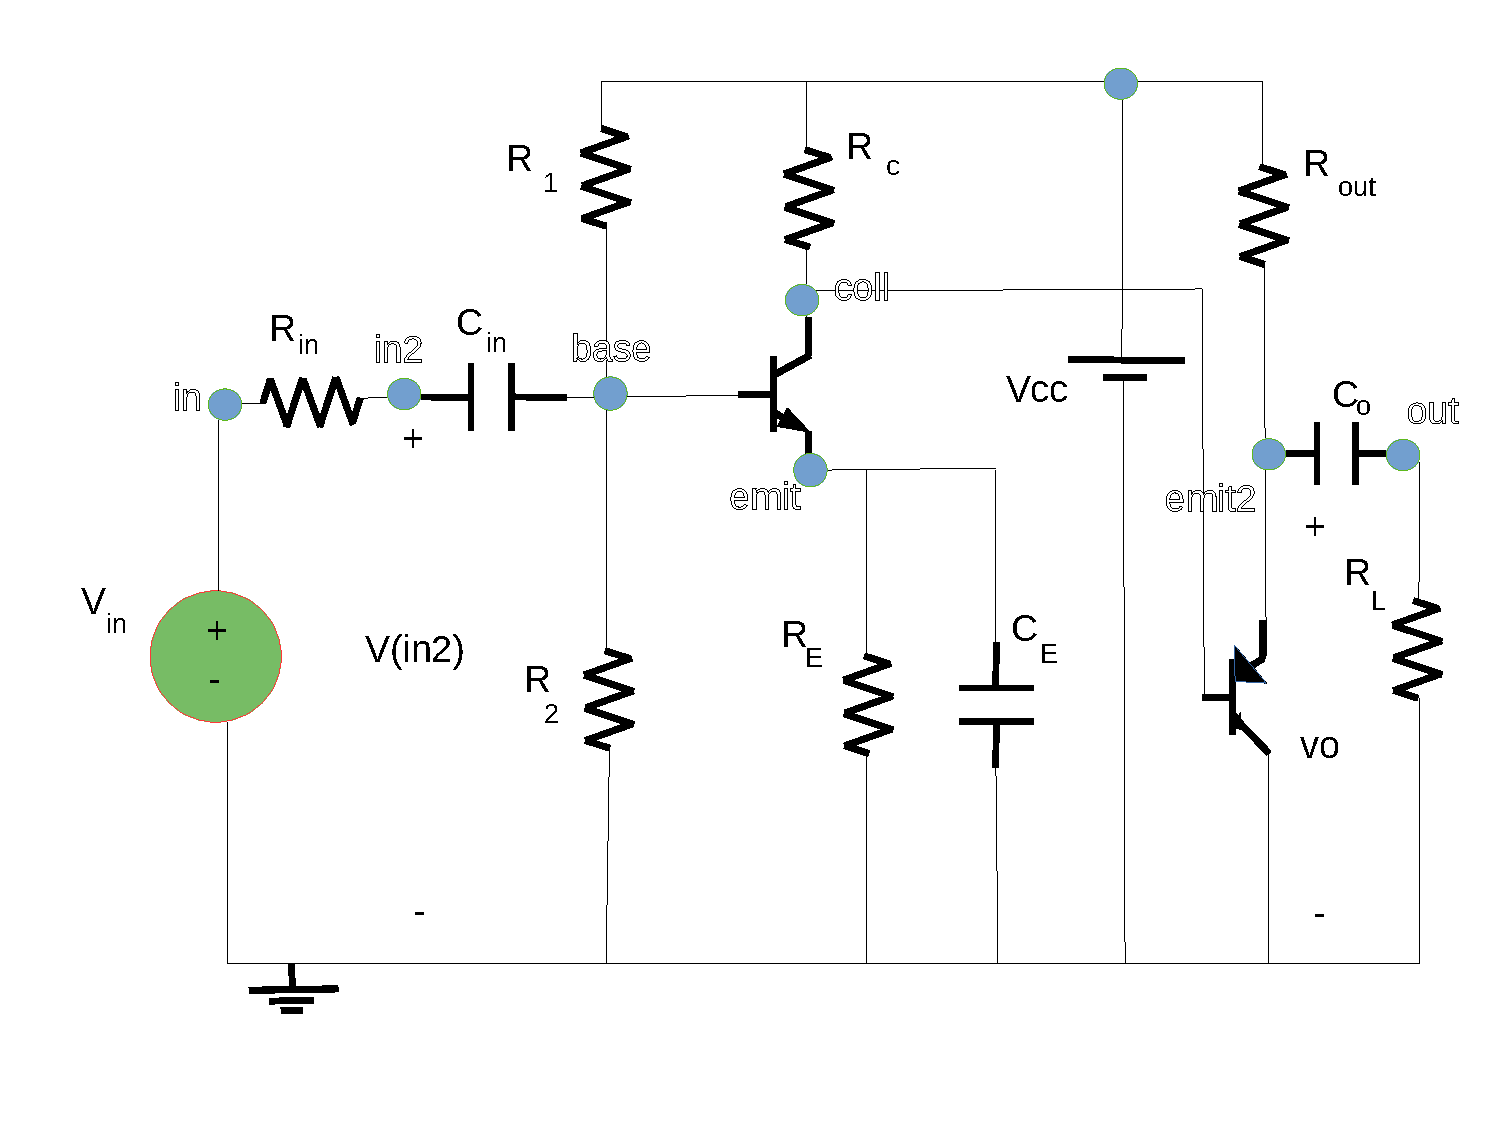
\includegraphics[width=1\linewidth]{lab4.pdf}
	\caption{Audio amplifier - given circuit}
	\label{fig:1}
\end{figure}

<<<<<<< HEAD
\par The input of this circuit is connected to an independent voltage source, which generates an ac signal with an amplitude of $10mV$. The source has an impedance of $100\Omega$, and the amplifier is going to be connected to a speaker which has an impedance of $8\Omega$. As we can see in the previous picture, the circuit is supplied by an independent 12V DC source (vcc).
\par The circuit comprises a gain stage and an output stage, which will be seen in a more detailed way in section \ref{sec:theoretical}. 
=======
\par As seen in the picture above, in this cirucit there was no sources used as the objetive of this assessment was to only build a circuit capable of amplifying any kind of signal and not a specific one. As such, vin and vout represent the input of the signal and its amplification, respectively. Through ngspice,  we were capable of measuring the wanted gain in the passband, the central frequency and the input and output impedances at the central frequency. In octave, a simulation of the circuit was also done with the required simplifications of the circuit. Gain, input and output impedances and frequency response were also obtained and then compared to the previously calculated on ngspice.

\par As seen in classes, an Op-Amp is a transistor based amplifier which is characterised by its high gain, high input impedance and low output impedance. For this laboratory assessment the group was given a list of components allowed to use and so the components used were all of them from this list.
>>>>>>> d0b080297fc0b7e965087175cb535c02ef7a19c1

\newpage
